
\subsection{Apprentissage automatique}

Dans un second temps, nous avons mis en place un système d'apprentissage automatique. C'est un algorithme de
classification qui permet de déterminer la classe d'un objet à partir de ses données. Il est basé
sur la notion de probabilité.

\vspace{0.5cm}

Tout d'abord nous importerons les bibliothèques nécessaires :

\begin{itemize}
    \item `sklearn` pour les algorithmes d'apprentissage automatique
    \item `numpy` pour les opérations mathématiques
    \item `pandas` pour les opérations sur les données
    \item `matplotlib` pour les graphiques
\end{itemize}

\vspace{0.5cm}

Ensuite nous allons importer et séparer les données :

À partir d’un échantillon de population qui représente nos données, on répartit les
données en deux groupes, les données d’entraînement et les données de test. La première
catégorie de données servira pendant la phase d’apprentissage du modèle alors que le
second sera utilisé pour évaluer la qualité de prédiction du modèle. Le but n’est donc
pas de construire une fonction qui prédira avec une précision optimale les valeurs des
variables cibles mais une fonction qui se généralisera au mieux pour prédire des valeurs
de données qui n’ont pas encore été observées.

\vspace{1.5cm}

\subsection{Régression}

Ici, pour déterminer la qualité du vin, nous allons mettre en place une régression.
Il s'agit d'un algorithme d’apprentissage supervisé c’est-à-dire qu’à partir de la
variable cible ou de la variable à expliquer (Y), le modèle a pour but de faire une
prédiction grâce à des variables dites explicatives (X) ou prédictives.

Nous avons tout d'abord défini le premier modèle. Il est composé de 4 couches composées
respectivement de 11 neurones en entrée, de 4 neurones chacunes pour les 2em et 3em couches
et 10 neurone pour la couche de sortie.

Avec cette configuration, nous avons défini un modèle de régression et obtenu
les résultats suivants :

\vspace{1cm}
\begin{figure}[!htb]

    \begin{minipage}{0.5\textwidth}
        \centering
        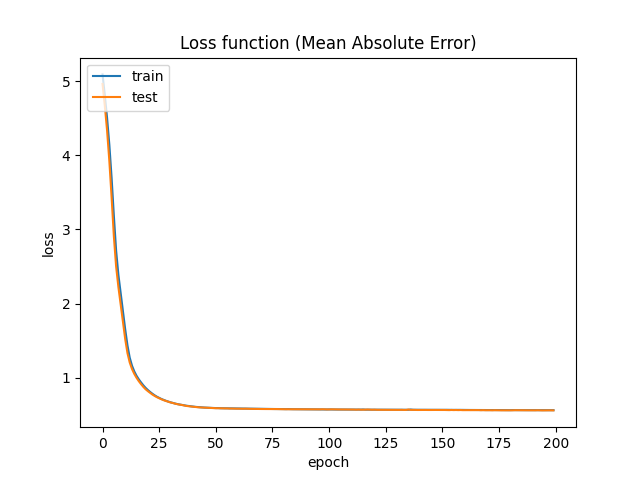
\includegraphics[width=01\textwidth]{../images/11-4-4/Loss_function(Mean_Absolute_Error).png}
        \label{fig:11-4-4-1}
    \end{minipage}\hfill

    \begin{minipage}{0.5\textwidth}
        \centering
        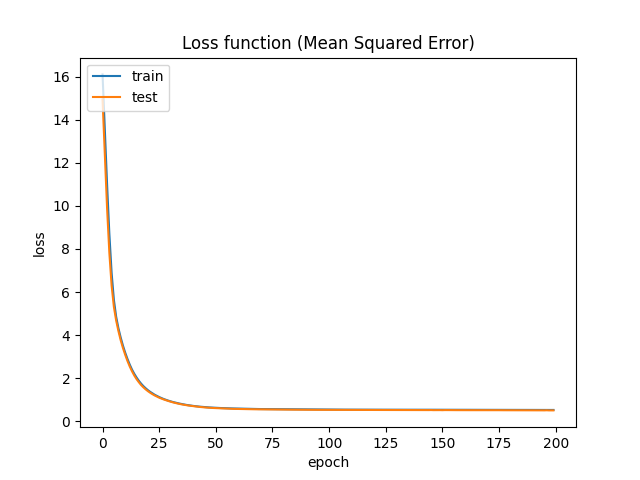
\includegraphics[width=01\textwidth]{../images/11-4-4/Loss_function(Mean_Squared_Error).png}
        \label{fig:11-4-4-1_squared}
    \end{minipage}\hfill

\end{figure}

\vspace{1cm}

On observe que les 2 courbes sont parfaitement superposées ce qui pourrait signifiee que notre réseau de neurones
ne fait aucune erreur. Mais en réalité, nous sommmes dans une situation de sous apprentissage. Pour y remédier, nous allons
complexifier le modèle en augmentant le nombre de neurones par couches.

On passe donc à la configuration suivante : 4 couches avec respectivement 11 neurones en entrée, 8 neurones sur les 2 couches
de traitement et 1 neurone de sortie.

\vspace{1cm}

\begin{figure}[!htb]
    \begin{minipage}{0.5\textwidth}
        \centering
        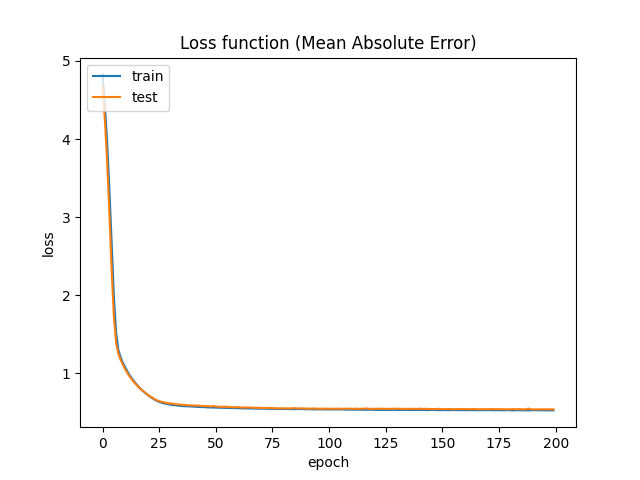
\includegraphics[width=01\textwidth]{../images/11-8-8/Loss_function(Mean_Absolute_Error).png}
        \label{fig:11-8-8-1.1}
    \end{minipage}\hfill
    \begin{minipage}{0.5\textwidth}
        \centering
        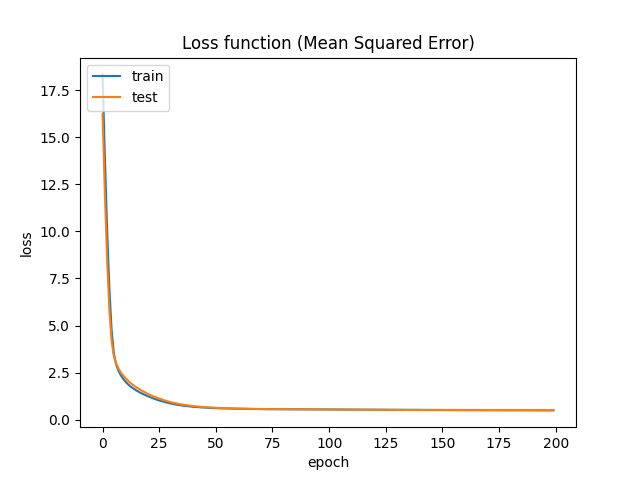
\includegraphics[width=01\textwidth]{../images/11-8-8/Loss_function(Mean_Squared_Error).png}
        \label{fig:11-8-8-1.1.2}
    \end{minipage}
    \caption{11-8-8-1}
\end{figure}

\vspace{1cm}
\newpage
On observe tout comme précédemment que les 2 courbes sont parfaitement superposées ce qui signifie que notre réseau de neurones
est toujours en sous apprentissage. Nous avons donc essayé de complexifier progressivement le modèle. En effet, nous avons
respectivement continué à augmenté le nombre de neurones par couches jusqu'à atteindre la configuration suivante : 11-20-20-1 puis ensuite
augmenté ne nombre de couches tout en continuant à varier le nombre de neurones par couches. Voici quelques exemples des résultats obtenus:

\vspace{1cm}
\begin{figure}[!htb]
    \begin{minipage}{0.5\textwidth}
        \centering
        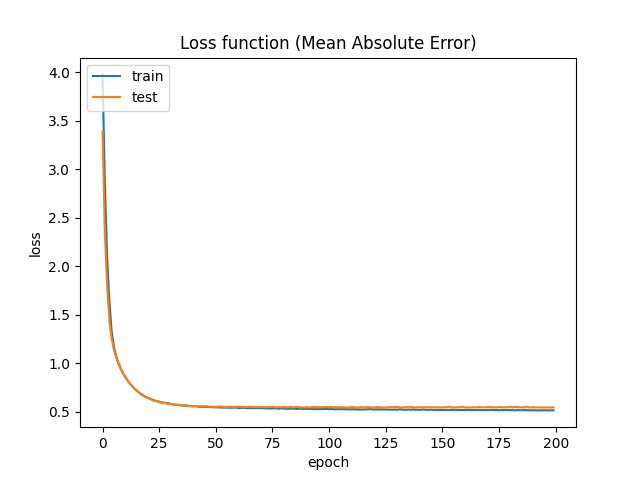
\includegraphics[width=01\textwidth]{../images/11-12-12/Loss_function(Mean_Absolute_Error).png}
        \label{fig:11-12-12-1.1}
    \end{minipage}\hfill
    \begin{minipage}{0.5\textwidth}
        \centering
        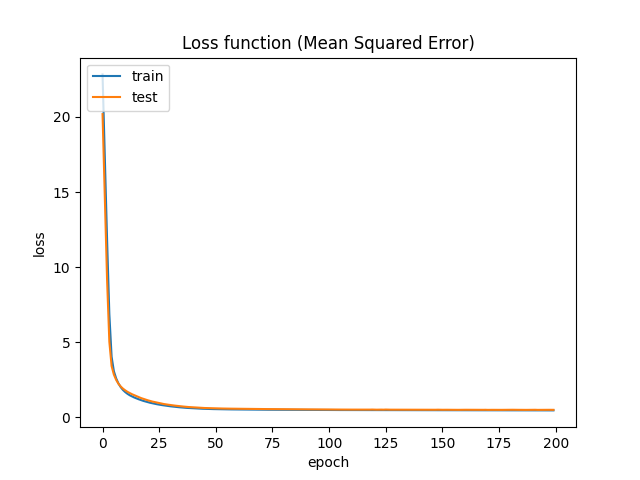
\includegraphics[width=01\textwidth]{../images/11-12-12/Loss_function(Mean_Squared_Error).png}
        \label{fig:11-12-12-1.1.2}
    \end{minipage}
    \caption{11-12-12-1}
\end{figure}

\begin{figure}[!htb]
    \begin{minipage}{0.5\textwidth}
        \centering
        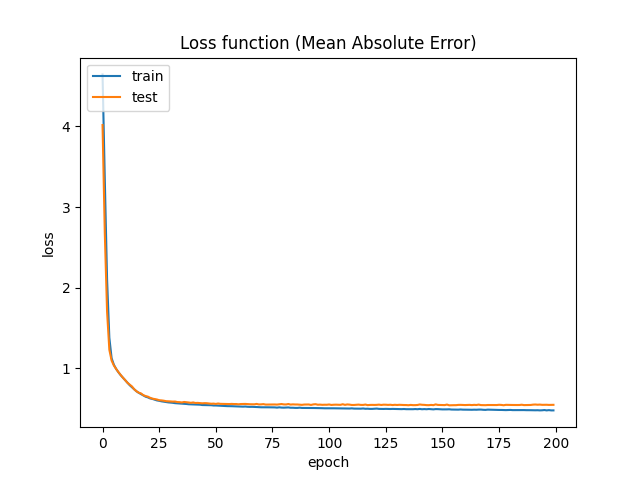
\includegraphics[width=01\textwidth]{../images/11-20-20/Loss_function(Mean_Absolute_Error).png}
        \label{fig:11-20-20-1.1}
    \end{minipage}\hfill
    \begin{minipage}{0.5\textwidth}
        \centering
        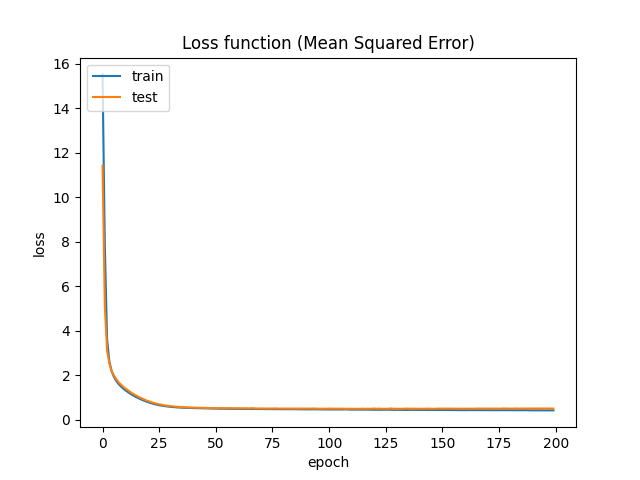
\includegraphics[width=01\textwidth]{../images/11-20-20/Loss_function(Mean_Squared_Error).png}
        \label{fig:11-20-20-1.1.2}
    \end{minipage}
    \caption{11-20-20-1}
\end{figure}

\vspace{1.5cm}

On observe donc que jusqu'à 2 couches de 20 neurones, notre modèle reste en sous apprentissage et commence tout juste à généraliser.
Ce n'est donc surement pas une bonne solution d'augmenter indéfiniment le nombre de neurones par couches.

Nous avons donc dessidé d'ajouter une troisième couche de neurones pour le traitement de l'information. Cette dernière contient le
même nombre de neurones les 2 couches précédentes. C'est avec cette nouvelle configuration que nous obtenons les résultats suivants pour
les nombres de neurones de 8, 12 et 20 :

\vspace*{1cm}

\begin{figure}[!htb]
    \begin{minipage}{0.5\textwidth}
        \centering
        \includegraphics[width=01\textwidth]{../images/11-8-8-8/Loss function(Mean Absolute Error).png}
        \label{fig:11-8-8-8-1.1}
    \end{minipage}\hfill
    \begin{minipage}{0.5\textwidth}
        \centering
        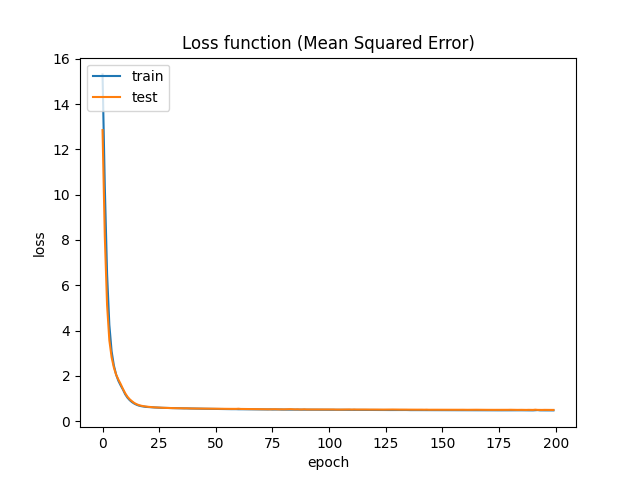
\includegraphics[width=01\textwidth]{../images/11-8-8-8/Loss function(Mean Squared Error).png}
        \label{fig:11-8-8-8-1.1.2}
    \end{minipage}
    \caption{11-8-8-8-1}
\end{figure}

\begin{figure}[!htb]
    \begin{minipage}{0.5\textwidth}
        \centering
        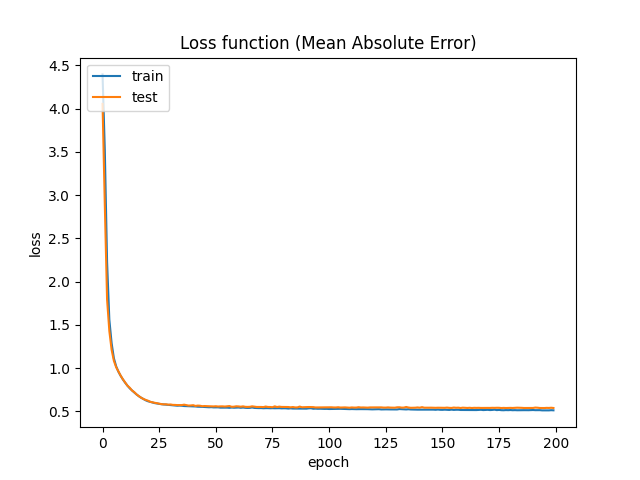
\includegraphics[width=01\textwidth]{../images/11-12-12-12/Loss function(Mean Absolute Error).png}
        \label{fig:11-12-12-12-1.1}
    \end{minipage}\hfill
    \begin{minipage}{0.5\textwidth}
        \centering
        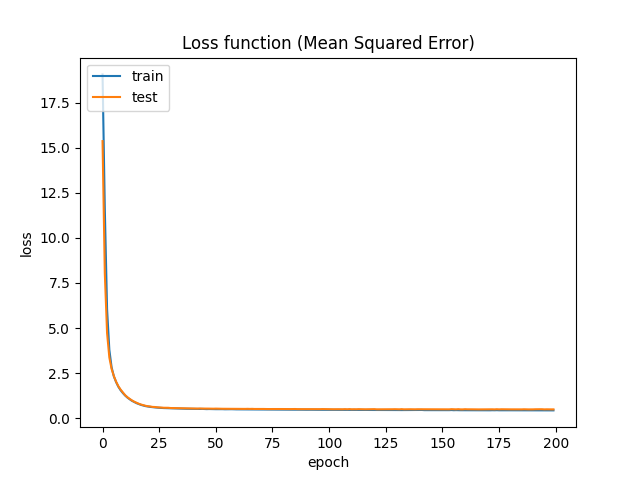
\includegraphics[width=01\textwidth]{../images/11-12-12-12/Loss function(Mean Squared Error).png}
        \label{fig:11-12-12-12-1.1.2}
    \end{minipage}
    \caption{11-12-12-12-1}
\end{figure}

\begin{figure}[!htb]
    \begin{minipage}{0.5\textwidth}
        \centering
        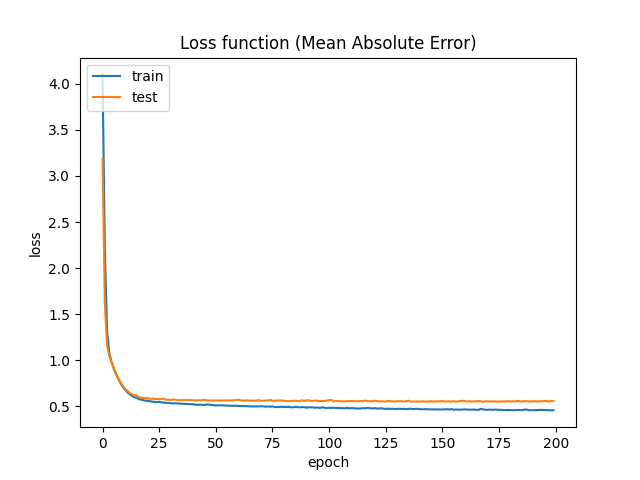
\includegraphics[width=01\textwidth]{../images/11-20-20-20/Loss function(Mean Absolute Error).png}
        \label{fig:11-20-20-20-1.1}
    \end{minipage}\hfill
    \begin{minipage}{0.5\textwidth}
        \centering
        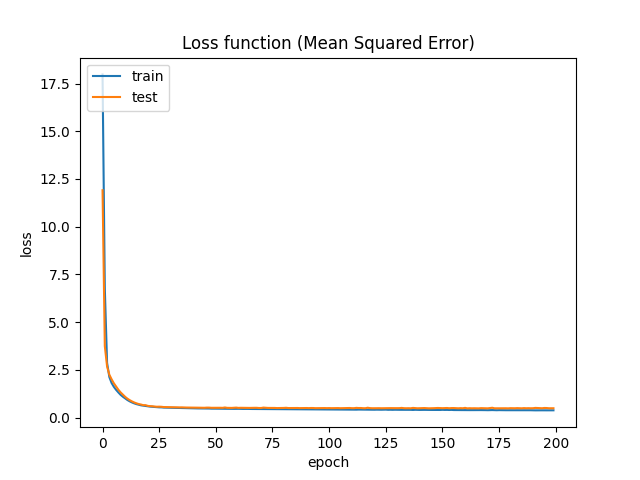
\includegraphics[width=01\textwidth]{../images/11-20-20-20/Loss function(Mean Squared Error).png}
        \label{fig:11-20-20-20-1.1.2}
    \end{minipage}
    \caption{11-20-20-20-1}
\end{figure}

\vspace{1cm}

Malgré tout notre modèle peine à généraliser. Nous aurions pu continuer à ajouter des couches et des neurones
pour tenter d'augmenter la précision du modèle. Mais nous avons cependant opté pour une réduction du nombre de
caractéristiques en entrée. Pour ce faire, nous avons tracé des histogrammes représentant à chaque fois
les valeurs prises par une caractéristique en fonction de la qualité du vin afin de déterminer si cette dernière (la caractéristique) est importante
dans la prédiction du résultat. Nous avons donc choisi de retirer les caractéristiques suivantes :

\newpage

\begin{itemize}
    \item le taux d'alcool
    \item la densité
    \item le dioxyde de soufre libre
\end{itemize}

\vspace{1cm}

Et obtenons les histogrammes suivants :

\vspace{1cm}

\begin{figure}[!htb]
    \begin{minipage}{0.5\textwidth}
        \centering
        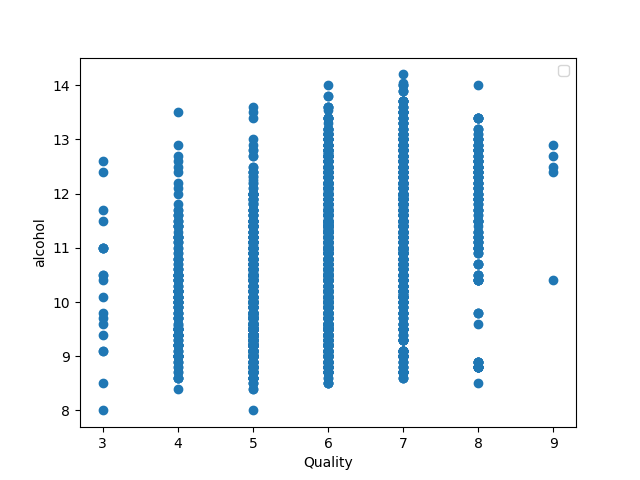
\includegraphics[width=01\textwidth]{../images/histo/alcohol.png}
        \label{fig:histogramme de l'alcool}
    \end{minipage}\hfill
    \begin{minipage}{0.5\textwidth}
        \centering
        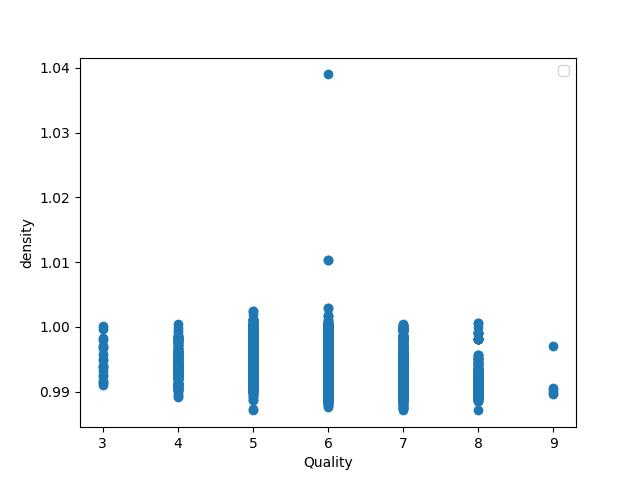
\includegraphics[width=01\textwidth]{../images/histo/density.png}
        \label{fig:histogramme de la densité}
    \end{minipage}
    \caption{Histogrammes de l'alcool et de la densité}
\end{figure}

\begin{figure}[!htb]
    \centering
    \begin{minipage}{0.5\textwidth}
        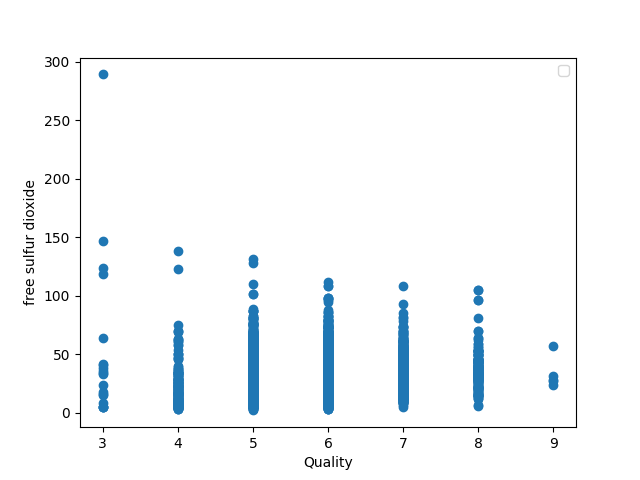
\includegraphics[width=01\textwidth]{../images/histo/free_sulfur_dioxide.png}
        \label{fig:histogramme du dioxyde de soufre libre}
    \end{minipage}\hfill

    \caption{histogramme du dioxyde de soufre libre}
\end{figure}

\newpage

Celà fait, nous avons retenté les mêmes expériences que précédemment, sans succès.

\vspace{1cm}

\begin{figure}[!htb]
    \begin{minipage}{0.5\textwidth}
        \centering
        \includegraphics[width=01\textwidth]{../images/bonnes_caractéristiques_suppr/8-8-8-8/Loss function(Mean Absolute Error).png}
        \label{fig:8-8-8-8-1.1}
    \end{minipage}\hfill
    \begin{minipage}{0.5\textwidth}
        \centering
        \includegraphics[width=01\textwidth]{../images/bonnes_caractéristiques_suppr/8-8-8-8/Loss function(Mean Squared Error).png}
        \label{fig:8-8-8-8-1.1.2}
    \end{minipage}
    \caption{8-8-8-8-1}
\end{figure}

\begin{figure}[!htb]
    \begin{minipage}{0.5\textwidth}
        \centering
        \includegraphics[width=01\textwidth]{../images/bonnes_caractéristiques_suppr/8-12-12-12/Loss function(Mean Absolute Error).png}
        \label{fig:8-12-12-12-1.1}
    \end{minipage}\hfill
    \begin{minipage}{0.5\textwidth}
        \centering
        \includegraphics[width=01\textwidth]{../images/bonnes_caractéristiques_suppr/8-12-12-12/Loss function(Mean Squared Error).png}
        \label{fig:8-12-12-12-1.1.2}
    \end{minipage}
    \caption{8-12-12-12-1}
\end{figure}

\begin{figure}[!htb]
    \begin{minipage}{0.5\textwidth}
        \centering
        \includegraphics[width=01\textwidth]{../images/bonnes_caractéristiques_suppr/8-20-20-20/Loss function(Mean Absolute Error).png}
        \label{fig:8-20-20-20-1.1}
    \end{minipage}\hfill
    \begin{minipage}{0.5\textwidth}
        \centering
        \includegraphics[width=01\textwidth]{../images/bonnes_caractéristiques_suppr/8-20-20-20/Loss function(Mean Squared Error).png}
        \label{fig:8-20-20-20-1.1.2}
    \end{minipage}
    \caption{8-20-20-20-1}
\end{figure}

\vspace{1cm}

Notre modèle n'a pas réussi à généraliser.
\newpage
